\chapter{\mypyvy}
\label{chap:mypyvy}

\section{Introduction}

Our experience with \Verdi and \disel has been
  that the most challenging aspect of distributed systems verification
  is discovering inductive invariants.
An inductive invariant is a property of system states that simultaneously
  (1) summarizes all the reachable states of the system,
  (2) is closed under all steps the system can take, and
  (3) ensures the absence of safety violations.
This challenge has led researchers to investigate 
  techniques for automatically inferring inductive invariants, 
  given a description of a system and its safety property.

This chapter describes \mypyvy
  a tool for automated reasoning
  about symbolic transition systems in first-order logic
  that supports a variety of automated reasoning tools to analyze systems.
\mypyvy takes an input file
  describing a symbolic transition system
  and performs the analysis requested by the user.
Three of the most interesting analyses include
  inductive invariant checking,
  inductive invariant inference, and
  bounded trace reasoning, including bounded model checking.
In all cases, \mypyvy loads the transition system
  and compiles it together with the user-requested analysis
  to a (sequence of) SMT queries,
  which are dispatched by Z3.

\mypyvy is not just the sum of the analyses currently available;
  it is a platform for doing research in automated verification.
We have ongoing projects that use the \mypyvy foundation
  to build several new invariant inference techniques 
  and user interfaces for verification and exploration.
In this context, \mypyvy can be seen as a sort of intermediate language
  that captures the right level of abstraction for implementing 
  invariant inference techniques.
Higher level languages, such as \ivy~\cite{Padon-al:PLDI16}
  that want to leverage invariant inference 
  can express their queries in \mypyvy and 
  use the available inference algorithms.
There is much exciting work to be done here. 
This chapter is more modest in scope, 
  describing the core of \mypyvy in theory and implementation.

\section{Background on Transition Systems and First-Order Logic}

\subsection{The robot example informally and pictorially}

\def\xMin{-8}
\def\xMax{8}
\def\yMin{-5}
\def\yMax{11}

\begin{figure}[t]
  \hfil%
  \begin{minipage}{0.45\linewidth}
    \centering
    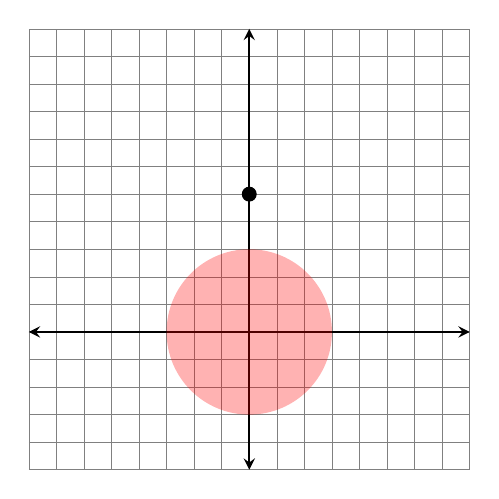
\begin{tikzpicture}[scale=0.35, >=stealth]
      \foreach \i in {\xMin,...,\xMax} {
          \draw [very thin,gray] (\i,\yMin) -- (\i,\yMax);
      }
      \foreach \i in {\yMin,...,\yMax} {
          \draw [very thin,gray] (\xMin,\i) -- (\xMax,\i);
      }
      \draw[<->, thick] (\xMin, 0) -- (\xMax, 0);
      \draw[<->, thick] (0, \yMin) -- (0, \yMax);
      \fill[fill=red, fill opacity=0.3] (0, 0) circle [radius=3];
      \draw[fill=black] (0, 5) circle [radius=0.25];
    \end{tikzpicture}
    \caption{Robot initial configuration.}
    \label{fig:robot-init}
  \end{minipage}%
  \hfil%
  \begin{minipage}{0.45\linewidth}
    \centering
    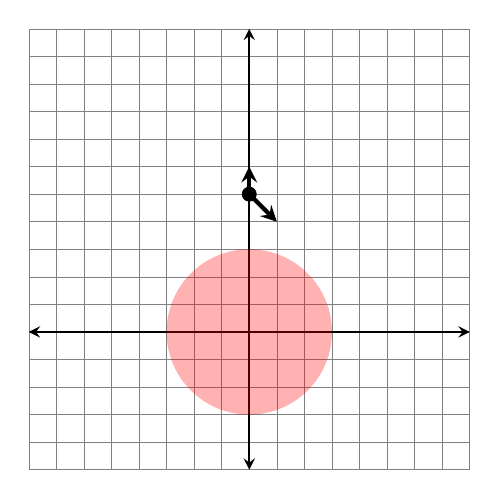
\begin{tikzpicture}[scale=0.35, >=stealth]
      \foreach \i in {\xMin,...,\xMax} {
          \draw [very thin,gray] (\i,\yMin) -- (\i,\yMax);
      }
      \foreach \i in {\yMin,...,\yMax} {
          \draw [very thin,gray] (\xMin,\i) -- (\xMax,\i);
      }
      \draw[<->, thick] (\xMin, 0) -- (\xMax, 0);
      \draw[<->, thick] (0, \yMin) -- (0, \yMax);
      \fill[fill=red, fill opacity=0.3] (0, 0) circle [radius=3];
      \draw[fill=black] (0, 5) circle [radius=0.25];
      \draw[->, line width=1.5pt] (0, 5) -- (0, 6);
      \draw[->, line width=1.5pt] (0, 5) -- (1, 4);
    \end{tikzpicture}
    \caption{Robot's first steps.}
    \label{fig:robot-first-steps}
  \end{minipage}%
  \hfil%
  \hrule
  \vspace{1em}
  \begin{minipage}{1\linewidth}
    \centering
    \begin{minipage}{0.5\linewidth}
      \centering
      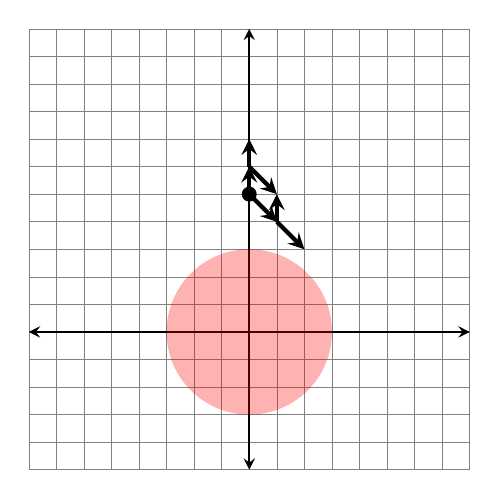
\begin{tikzpicture}[scale=0.35, >=stealth]
        \foreach \i in {\xMin,...,\xMax} {
            \draw [very thin,gray] (\i,\yMin) -- (\i,\yMax);
        }
        \foreach \i in {\yMin,...,\yMax} {
            \draw [very thin,gray] (\xMin,\i) -- (\xMax,\i);
        }
        \draw[<->, thick] (\xMin, 0) -- (\xMax, 0);
        \draw[<->, thick] (0, \yMin) -- (0, \yMax);
        \fill[fill=red, fill opacity=0.3] (0, 0) circle [radius=3];
        \draw[fill=black] (0, 5) circle [radius=0.25];
        \draw[->, line width=1.5pt] (0, 5) -- (0, 6);
        \draw[->, line width=1.5pt] (0, 5) -- (1, 4);
        \draw[->, line width=1.5pt] (0, 6) -- (0, 7);
        \draw[->, line width=1.5pt] (0, 6) -- (1, 5);
        \draw[->, line width=1.5pt] (1, 4) -- (1, 5);
        \draw[->, line width=1.5pt] (1, 4) -- (2, 3);
      \end{tikzpicture}%
    \end{minipage}%
    \begin{minipage}{0.5\linewidth}
      \centering
      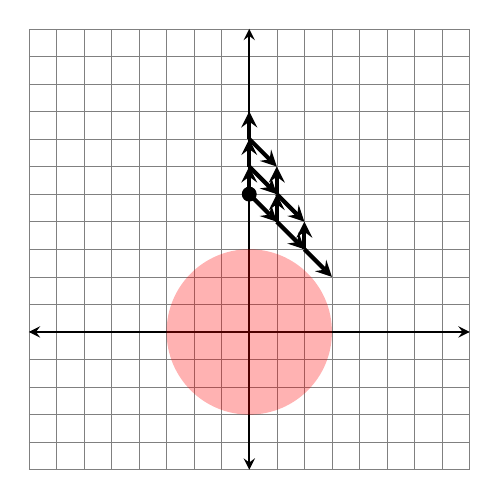
\begin{tikzpicture}[scale=0.35, >=stealth]
        \foreach \i in {\xMin,...,\xMax} {
            \draw [very thin,gray] (\i,\yMin) -- (\i,\yMax);
        }
        \foreach \i in {\yMin,...,\yMax} {
            \draw [very thin,gray] (\xMin,\i) -- (\xMax,\i);
        }
        \draw[<->, thick] (\xMin, 0) -- (\xMax, 0);
        \draw[<->, thick] (0, \yMin) -- (0, \yMax);
        \fill[fill=red, fill opacity=0.3] (0, 0) circle [radius=3];
        \draw[fill=black] (0, 5) circle [radius=0.25];
        \draw[->, line width=1.5pt] (0, 5) -- (0, 6);
        \draw[->, line width=1.5pt] (0, 5) -- (1, 4);
        \draw[->, line width=1.5pt] (0, 6) -- (0, 7);
        \draw[->, line width=1.5pt] (0, 6) -- (1, 5);
        \draw[->, line width=1.5pt] (1, 4) -- (1, 5);
        \draw[->, line width=1.5pt] (1, 4) -- (2, 3);
        \draw[->, line width=1.5pt] (0, 7) -- (0, 8);
        \draw[->, line width=1.5pt] (0, 7) -- (1, 6);
        \draw[->, line width=1.5pt] (1, 5) -- (1, 6);
        \draw[->, line width=1.5pt] (1, 5) -- (2, 4);
        \draw[->, line width=1.5pt] (2, 3) -- (2, 4);
        \draw[->, line width=1.5pt] (2, 3) -- (3, 2);
      \end{tikzpicture}
    \end{minipage}%
    \caption{Robot's second and third steps.}
    \label{fig:robot-23-steps}
  \end{minipage}
\end{figure}

Imagine robot in a 2-dimensional world.
The robot starts at position $(0, 5)$,
  and can take steps to integer grid points either
 due north or diagonally southeast of its current position.
The world has a circular hole of radius 3 centered at the origin.
Can the robot ever fall in the hole?\footnote{Thanks to Jon Howell for this example.}

The initial situation is depicted in \cref{fig:robot-init}.
The smaller black circle represents the robot's initial position,
  and the larger shaded red circle represents the hole at the origin.
In its first step, shown in \cref{fig:robot-first-steps},
  the robot could either move north one square,
  or diagonally southeast one square.
These two possibilities are drawn as thick black arrows.
So far, the robot manages to avoid falling in.

As the robot progresses, more and more positions are reachable,
  each with a sequence of moves due north or diagonally southeast.
The set of possible positions after two and three steps
  are shown in \cref{fig:robot-23-steps}.
Despite the growing number of reachable positions,
  no sequence of steps causes the robot to fall in.

\begin{figure}[t]
  \hfil%
  \begin{minipage}{0.45\linewidth}
    \centering
    \begin{tikzpicture}[scale=0.35, >=stealth]
      \foreach \i in {\xMin,...,\xMax} {
          \draw [very thin,gray] (\i,\yMin) -- (\i,\yMax);
      }
      \foreach \i in {\yMin,...,\yMax} {
          \draw [very thin,gray] (\xMin,\i) -- (\xMax,\i);
      }
      \draw[<->, thick] (\xMin, 0) -- (\xMax, 0);
      \draw[<->, thick] (0, \yMin) -- (0, \yMax);
      \fill[fill=red, fill opacity=0.3] (0, 0) circle [radius=3];
      \draw[fill=black] (0, 5) circle [radius=0.25];
      \fill[fill=green, fill opacity=0.3] (0, 5) -- (0, \yMax) -- (\xMax, \yMax) -- ($(\xMax,5)-(0,\xMax)$) -- cycle;
    \end{tikzpicture}
    \caption{Exact characterization of the robot's reachable positions.}
    \label{fig:robot-reachable}
  \end{minipage}%
  \hfil%
  \begin{minipage}{0.45\linewidth}
    \centering
    \begin{tikzpicture}[scale=0.35, >=stealth]
      \foreach \i in {\xMin,...,\xMax} {
          \draw [very thin,gray] (\i,\yMin) -- (\i,\yMax);
      }
      \foreach \i in {\yMin,...,\yMax} {
          \draw [very thin,gray] (\xMin,\i) -- (\xMax,\i);
      }
      \draw[<->, thick] (\xMin, 0) -- (\xMax, 0);
      \draw[<->, thick] (0, \yMin) -- (0, \yMax);
      \fill[fill=red, fill opacity=0.3] (0, 0) circle [radius=3];
      \draw[fill=black] (0, 5) circle [radius=0.25];
      \fill[fill=blue, fill opacity=0.3] (0, 5) -- ($(-\yMax,\yMax)+(5,0)$) -- (\xMax, \yMax) -- ($(\xMax,5)-(0,\xMax)$) -- cycle;
    \end{tikzpicture}
    \caption{A simple overapproximation to the set of reachable positions.}
    \label{fig:robot-inductive-invariant}
  \end{minipage}
  \hfil%
\end{figure}

We start to see a pattern emerging.
No matter what happens,
  the robot will never be able to move west of the $y$ axis,
  nor will it be able to move southwest
    of the diagonal line $x + y = 5$.
This region is shown shaded in green in \cref{fig:robot-reachable}.
Visually, this green polygonal region does not overlap with the red circle,
  which ``proves'' that the robot never falls in.

In fact, this green region exactly characterizes
  the set of possible positions that the robot could reach
  through some sequence of moves.
(We call such positions ``reachable''.)
Given any point in the green region,
  the robot can reach it by first moving southeast over and over until
  it is vertically below the target point,
  and then moving due north over and over until the point is reached.

Our proof that the robot never falls in
  can be simplified slightly be noticing
  that we never used the fact that
  the robot always remains east of the $y$ axis.
Instead, it is enough to convince ourselves that
  the robot is always northeast of the line $x + y = 5$.
This region is shown in blue in \cref{fig:robot-inductive-invariant}.
Again, it does not visually overlap with the circle,
  so it constitutes a visual ``proof'' that the robot never falls in.

This time, though, not every position in the blue polygonal region is reachable,
  since we have already realized that no position west of the $y$ axis is reachable.
The unreachable positions from this region are shown in \cref{fig:robot-unreachable}.
This second proof demonstrates that we can prove the robot never falls in
  even without exactly characterizing the set of reachable positions.

\begin{figure}[t]%
%  \centering%
  \hfil%
  \begin{minipage}{0.45\linewidth}
    \centering
    \begin{tikzpicture}[scale=0.35, >=stealth]
      \foreach \i in {\xMin,...,\xMax} {
          \draw [very thin,gray] (\i,\yMin) -- (\i,\yMax);
      }
      \foreach \i in {\yMin,...,\yMax} {
          \draw [very thin,gray] (\xMin,\i) -- (\xMax,\i);
      }
      \draw[<->, thick] (\xMin, 0) -- (\xMax, 0);
      \draw[<->, thick] (0, \yMin) -- (0, \yMax);
      \fill[fill=red, fill opacity=0.3] (0, 0) circle [radius=3];
      \draw[fill=black] (0, 5) circle [radius=0.25];
      \fill[fill=yellow, fill opacity=0.3] (-1, 5) -- (-1, \yMax) -- ($(-\yMax,\yMax)+(5,0)$) -- cycle;
    \end{tikzpicture}
    \caption{Positions from \cref{fig:robot-inductive-invariant} that are unreachable.}
    \label{fig:robot-unreachable}
  \end{minipage}%
  \hfil%
  \begin{minipage}{0.45\linewidth}
    \centering
    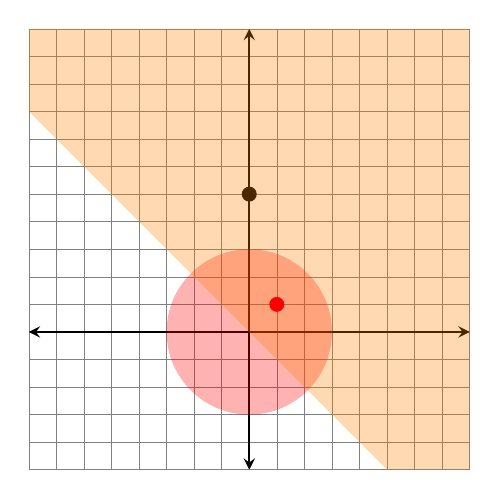
\begin{tikzpicture}[scale=0.35, >=stealth]
      \foreach \i in {\xMin,...,\xMax} {
          \draw [very thin,gray] (\i,\yMin) -- (\i,\yMax);
      }
      \foreach \i in {\yMin,...,\yMax} {
          \draw [very thin,gray] (\xMin,\i) -- (\xMax,\i);
      }
      \draw[<->, thick] (\xMin, 0) -- (\xMax, 0);
      \draw[<->, thick] (0, \yMin) -- (0, \yMax);
      \fill[fill=red, fill opacity=0.3] (0, 0) circle [radius=3];
      \draw[fill=black] (0, 5) circle [radius=0.25];
      \fill[fill=orange, fill opacity=0.3]
      (\xMin, -\xMin) -- (\xMin, \yMax) -- (\xMax, \yMax) -- (\xMax, \yMin) --
      (-\yMin, \yMin) -- cycle;
      \draw[red,fill=red] (1, 1) circle [radius=0.25];
    \end{tikzpicture}
    \caption{The orange region is unsafe because it intersects the red circle.}
    \label{fig:robot-unsafe}
  \end{minipage}%
%  \dotfill
  \hfil
\end{figure}

\begin{figure}[t]
  \centering
\end{figure}

Reflecting on our two admittedly informal proofs so far,
  we can boil them each down into three essential proof steps:
  (1) identify a set of positions $I$ that
  (2) contains all reachable positions; and that
  (3) does not intersect the red circle.
Each proof step is important.
Proof step (1) requires some creativity and foresight
  to pick a set that will make proof steps (2) and (3) possible.
Proof step (3) has been fairly straightforward so far,
  because we can visually analyze our set and the red circle
  to determine if they overlap.
If we wanted to be more precise about proof step (3),
  we could do some algebra to show that
  any position $(x, y)$ that satisfies the linear inequalities
  that define the polygonal regions from
    \cref{fig:robot-reachable,fig:robot-inductive-invariant}
  always fall outside the red circle,
  i.e. $\sqrt{x^2 + y^2} > 3$.

Proof step (2) is more subtle.
We have claimed informally that the robot will never
  be able to move southwest of the line $x + y = 5$,
  nor west of the $y$ axis,
  but what would constitute a more detailed proof of this fact?
These claims are claims of \emph{invariance},
  i.e., that the set $I$ from proof step (1) is an invariant,
  where an invariant is a set that contains all reachable positions.
The key to proving invariance is an \emph{inductive} argument,
  which first shows (2.1) that the initial position is in $I$
  and then shows (2.2) that, from any position in $I$,
  all steps the robot could take
  lead to new positions that are also in $I$.
By induction, this implies that all reachable positions
  are contained in $I$.
For the invariants represented in
  \cref{fig:robot-reachable,fig:robot-inductive-invariant}
  we could make proof steps (2.1) and (2.2) more precise
  by showing that the initial position
    satisfies the linear inequalities for the polygonal regions
  and by showing that if $(x,y)$ satisfies the inequalities,
    then so do both $(x, y+1)$ (moving due north)
      and $(x+1, y-1)$ (moving southeast).

\begin{figure}[t]%
%  \centering%
  \hfil%
  \begin{minipage}{0.45\linewidth}
    \centering
      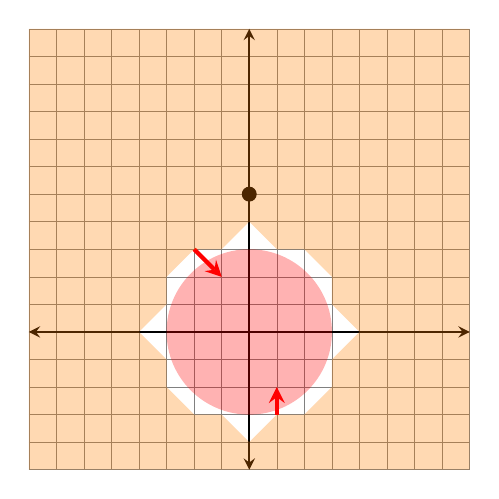
\begin{tikzpicture}[scale=0.35, >=stealth]
        \foreach \i in {\xMin,...,\xMax} {
            \draw [very thin,gray] (\i,\yMin) -- (\i,\yMax);
        }
        \foreach \i in {\yMin,...,\yMax} {
            \draw [very thin,gray] (\xMin,\i) -- (\xMax,\i);
        }
        \draw[<->, thick] (\xMin, 0) -- (\xMax, 0);
        \draw[<->, thick] (0, \yMin) -- (0, \yMax);
        \fill[fill=red, fill opacity=0.3] (0, 0) circle [radius=3];
        \draw[fill=black] (0, 5) circle [radius=0.25];
        \draw[red, ->, line width=1.5pt] (-2, 3) -- +(1, -1);
        \draw[red, ->, line width=1.5pt] (1, -3) -- +(0, 1);
        \fill[even odd rule, fill=orange, fill opacity=0.3]
        (0, 4) -- ++(1, -1) -- ++(1, 0) -- ++(1, -1) -- ++(0, -1) -- ++(1, -1)
               -- ++(-1, -1) -- ++(0, -1) -- ++(-1, -1) -- ++(-1, 0) -- ++(-1, -1)
               -- ++(-1, 1) -- ++(-1, 0) -- ++(-1, 1) -- ++(0, 1) -- ++(-1, 1)
               -- ++(1, 1) -- ++(0, 1) -- ++(1, 1) -- ++(1, 0) -- ++(1, 1)
               -- cycle
        (\xMin, \yMax) -- (\xMax, \yMax) -- (\xMax, \yMin) -- (\xMin, \yMin) -- cycle;
      \end{tikzpicture}
    \caption{The region outside the circle is invariant but not inductive.}
    \label{fig:robot-cti1}
  \end{minipage}%
  \hfil%
  \begin{minipage}{0.45\linewidth}
    \centering
    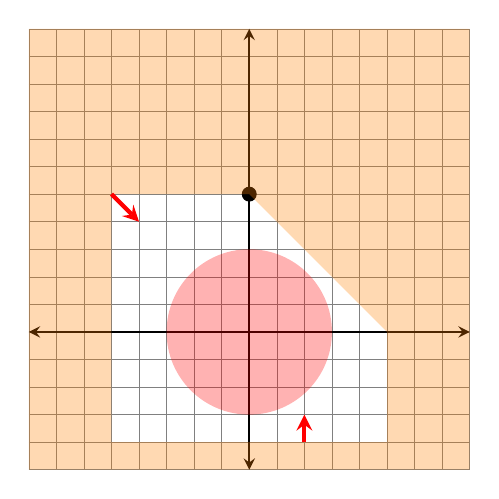
\begin{tikzpicture}[scale=0.35, >=stealth]
      \foreach \i in {\xMin,...,\xMax} {
          \draw [very thin,gray] (\i,\yMin) -- (\i,\yMax);
      }
      \foreach \i in {\yMin,...,\yMax} {
          \draw [very thin,gray] (\xMin,\i) -- (\xMax,\i);
      }
      \draw[<->, thick] (\xMin, 0) -- (\xMax, 0);
      \draw[<->, thick] (0, \yMin) -- (0, \yMax);
      \fill[fill=red, fill opacity=0.3] (0, 0) circle [radius=3];
      \draw[fill=black] (0, 5) circle [radius=0.25];
      \fill[even odd rule, fill=orange, fill opacity=0.3]
      (0, 5) -- (5, 0) -- (5, -4) -- (-5, -4) -- (-5, 5) -- cycle
      (\xMin, \yMax) -- (\xMax, \yMax) -- (\xMax, \yMin) -- (\xMin, \yMin) -- cycle;
      \draw[red, ->, line width=1.5pt] (-5, 5) -- (-4, 4);
      \draw[red, ->, line width=1.5pt] (2, -4) -- +(0, 1);
    \end{tikzpicture}
    \caption{This simplified region is also invariant but not inductive.}
    \label{fig:robot-cti2}
  \end{minipage}%
%  \dotfill
  \hfil
\end{figure}

It is instructive to see what happens when
  the set $I$ selected in proof step (1)
  fails to proof steps (2) or (3).
When proof step (3) fails,
  $I$ intersects the red circle,
  as in \cref{fig:robot-unsafe}.
In this case we call the set $I$ ``unsafe''.
The small opaque red dot shows an example position that is both
  in the candidate set $I$ drawn as the orange region
  and the shaded red circle at the origin.
When proof step (2) fails,
  there is a position in $I$ from which
  the robot can step to a position outside $I$,
  as in \cref{fig:robot-cti1,fig:robot-cti2}.
The red arrows show examples of positions in the orange regions
  that can step out of orange regions.
We call such positions ``counterexamples to inductiveness'', or CTIs.

\begin{figure}[t]%
  \hfil%
  \begin{minipage}{0.45\linewidth}
    \centering
    \begin{tikzpicture}[scale=0.35, >=stealth]
      \foreach \i in {\xMin,...,\xMax} {
          \draw [very thin,gray] (\i,\yMin) -- (\i,\yMax);
      }
      \foreach \i in {\yMin,...,\yMax} {
          \draw [very thin,gray] (\xMin,\i) -- (\xMax,\i);
      }
      \draw[<->, thick] (\xMin, 0) -- (\xMax, 0);
      \draw[<->, thick] (0, \yMin) -- (0, \yMax);
      \fill[fill=red, fill opacity=0.3] (0, 0) circle [radius=3];
      \draw[fill=black] (0, 5) circle [radius=0.25];
      \fill[fill=violet, fill opacity=0.4] (0, 5) -- (3, 2) -- (3, 1) -- (4, 0) -- (4, \yMin) -- (\xMax, \yMin) -- (\xMax, \yMax) -- ($(-\yMax,\yMax)+(5,0)$) -- cycle;
    \end{tikzpicture}
    \caption{The largest safe inductive invariant for the robot.}
    \label{fig:robot-large-invariant}
  \end{minipage}%
  \hfil%
  \begin{minipage}{0.45\linewidth}
    \centering
    \begin{tikzpicture}[scale=0.35, >=stealth]
      \foreach \i in {\xMin,...,\xMax} {
          \draw [very thin,gray] (\i,\yMin) -- (\i,\yMax);
      }
      \foreach \i in {\yMin,...,\yMax} {
          \draw [very thin,gray] (\xMin,\i) -- (\xMax,\i);
      }
      \draw[<->, thick] (\xMin, 0) -- (\xMax, 0);
      \draw[<->, thick] (0, \yMin) -- (0, \yMax);
      \fill[fill=red, fill opacity=0.3] (0, 0) circle [radius=3];
      \draw[fill=black] (0, 5) circle [radius=0.25];
      \fill[fill=violet, fill opacity=0.4] (0, 5) -- (3, 2) -- (3, 1) -- (4, 0) -- (4, \yMin) -- (\xMax, \yMin) -- (\xMax, \yMax) -- ($(-\yMax,\yMax)+(5,0)$) -- cycle;
      \draw[->, red, line width=1.5pt] ($(-\yMax,\yMax)+(4,0)$) -- (2, 2);
      \draw[->, red, line width=1.5pt] (3, \yMin) -- (3, 0);
    \end{tikzpicture}
    \caption{Proof that every position outside the purple region is backward reachable.}
    \label{fig:robot-backward-reachable}
  \end{minipage}%
  \hfil
\end{figure}

In the robot example, we can rephrase inductiveness by saying:
  if a position $(x, y)$ is \emph{not} in $I$,
  then neither is any state due south or diagonally northwest of $(x, y)$.
Since our goal in any proof of the robot's safety is
  to come up with a set $I$ that is inductive and does not intersect the red circle,
  we know the states in the red circle must not be in $I$.
Using the rephrasing above,
  we can conclude that $I$ must also not contain
  any state due south or diagonally northwest of the red circle.
Continuing to rule out states in this way,
  we can find the \emph{largest} set $I$ that will make the proof go through,
  shown in \cref{fig:robot-large-invariant}.
To convince ourselves that this region $I$ is the largest safe inductive invariant,
  it is enough to show that every position not in $I$ is \emph{backward reachable},
  by which we mean, there is a sequence of steps
  starting from the position and ending somewhere in the red circle.
\Cref{fig:robot-backward-reachable} demonstrates that
  the positions just outside the purple region are all backward reachable,
  using sequences of steps that follow the red arrows to the red circle.
Every other position outside the purple shaded region
  is either due south or diagonally northwest of one of these two red arrows,
  and so is also backward reachable.

Because the robot example is so simple,
  we are able to exactly characterize
    the set of reachable states (\cref{fig:robot-reachable}) and
    the set of backward reachable states (\cref{fig:robot-backward-reachable}).
In more complex examples, this will be much more difficult,
  but luckily it will always be sufficient to find an overapproximation
  to the set of reachable states, such as \cref{fig:robot-inductive-invariant},
  which proves safety without exactly characterizing
  reachability or backward reachability.

\subsection{The robot example in set theory}

\def\robot{\ensuremath{\mathsf{robot}}}
\def\reach{\ensuremath{\mathsf{reach}}}

Let's formalize the robot example from the previous section
  using the language of set theory.

A \emph{transition system} $\tau = (S, S^0, \to)$ consists of a set of states $S$,
  a set of initial states $S^0\subseteq S$,
  and a binary transition relation $\to\subseteq S\times S$.
We write $s\to s'$ to mean $(s, s') \in \to$.

We can formalize the robot example as a transition system as follows.
\begin{align*}
  \tau_\robot &= (S_\robot, S^0_\robot, \to_\robot)\\
  S_\robot &= \set{(x,y) \mid x,y\in\Z}\\
  S^0_\robot &= \set{(0, 5)}\\
  \to_\robot &= \set{((x,y), (x, y + 1)) \mid x,y\in\Z} \mathrel{\cup}\\
            &\phantom{\mathrel{=}}\quad \set{((x,y), (x + 1, y - 1)) \mid x,y\in\Z}
\end{align*}

We write $s\to^* s'$ to mean that there is a (possibly empty) sequence of steps from $s$ to $s'$.
Using this notation, we can say that a state $s$ is \emph{reachable}
  if there is an initial state $s_0\in S^0$ such that $s_0 \to^* s$.
We write $\reach(\tau)$ for the set of reachable states of the transition system $\tau$.

In the robot example,
  we characterized the set of reachable states in \cref{fig:robot-reachable}.
We can express the set precisely as
\[
  \reach(\tau_\robot) = \set{(x,y) \mid x \ge 0 \text{ and } x + y \ge 5}
\]
The proof of this fact follows the informal discussion from the previous section.
First, the set on the right hand side contains all reachable states,
  which can be shown with an inductive argument (that we spell out below).
Second, every state in this set is reachable,
  which we can show by
  first showing that everything on the diagonal $x + y = 5 \land x \ge 0$ is reachable
    (by a sequence of southeast moves from the initial state),
  and then showing that every state above the diagonal is reachable
    (by a subsequent sequence of north moves).

In the robot example, our goal was to prove the robot never falls in the red circle.
In general, the kinds of goals we will be interested in will be \emph{safety properties},
  specifically, that a transition system avoids a certain set of \emph{bad states} $B\subseteq S$
  that is claimed not to intersect the set of reachable states.
In the robot example, the bad states are the ones in the red circle:
\[
  B_\robot = \set{(x,y) \mid \sqrt{x^2 + y^2} \le 3}.
\]
The claim that the robot is \emph{safe} means that $B_\robot$ does not intersect $\reach(\tau_\robot)$,
  which is visually apparent in \cref{fig:robot-reachable}.

In simple systems, such as the robot example,
  $\reach(\tau)$ can be characterized directly,
  but in more complex systems, it is neither practical nor useful
  to obtain an exact characterization of reachable states.
Instead, one often uses \emph{overapproximations} to reachability,
  known as invariants.
We say that a set $I$ is an \emph{invariant} if it contains every reachable state,
  that is, if $\reach(\tau) \subseteq I$.
Thus, another way to talk about safety properties is to say that
  the complement of the set of bad states is an invariant,
  i.e. $\reach(\tau) \subseteq S\setminus B$.
Indeed, another way to set up the safety verification problem is
  to specify $S\setminus B$ directly instead of $B$,
  and to claim that $S\setminus B$ is an invariant.
We call this the \emph{positive phrasing of the safety problem}.

When $\reach(\tau)$ has a direct characterization,
  one can prove that $I$ is an invariant directly from the definition.
But in complex systems where
  no useful direct characterization of $\reach(\tau)$ exists,
  one instead uses an inductive argument to establish invariance.
We say that $I$ is an \emph{inductive invariant} if:
  (1) $S^0\subseteq I$; and
  (2) for any $s\in I$, if $s\to s'$, then $s' \in I$.

Both the green region from \cref{fig:robot-reachable} and
  the blue region from \cref{fig:robot-inductive-invariant}
  are invariants, and in fact are inductive invariants.
(Indeed $\reach(\tau)$ is always an inductive invariant in any transition system.)
However, not all invariants are inductive invariants.
For example, the orange regions from \cref{fig:robot-cti1,fig:robot-cti2}
  are both invariants (because they contain the green region from \cref{fig:robot-reachable})
  but neither are inductive.
If we wanted to use an inductive argument to show
  that these orange regions are invariants,
  we would need to first \emph{strengthen} them.

In general, suppose we want to prove that $I$ is an invariant of some transition system $\tau$,
  and that we don't have a useful direct characterization of $\reach(\tau)$ handy.
Further, suppose that $I$ is not inductive.
To show that $I$ is an invariant, it is enough to find another set $J$ such that:
  (1) $J\subseteq I$; and
  (2) $J$ is inductive.
Since $J$ is inductive, $J$ is an invariant, i.e. $\reach(\tau)\subseteq J$.
But $J\subseteq I$, so $I$ is also an invariant.
In the robot example, we could use the blue region from \cref{fig:robot-inductive-invariant}
  as an inductive strengthening
  to prove that either of the orange regions is an invariant.
Most of the art and skill of working with transition systems
  is in the ability to look at a non-inductive property
  and see what kinds of strengthenings of it
  might be good ideas to get it to be inductive.

\subsection{Background on first-order logic}

\begin{verbatim}
  - sorts
  - relations, constants, and functions; signatures
  - syntax of FOL
  - FO-structures over a signature
  - interpreting syntax in a structure; defn of "model"
  - EPR: definition and model theory 
  - extensions to EPR: stratified functions
\end{verbatim}

Many of the ideas of first-order logic are not complicated,
  but they are tedious to set up formally.
In this section, we do our best.

A \emph{sort} is either $\mathbb{B}$ or an uninterpreted symbol.

A \emph{function type} is some number of argument sorts and a return sort.

A \emph{vocabulary} is a map from names to function types

A \emph{first-order structure} over a vocabulary is 
  a set for every uninterpreted sort symbol


\subsection{First-order logic for transition systems}

We are on a journey to more and more formally specify the robot example
  and to prove its safety more and more automatically.
The next step on this journey is through first-order logic,
  which we assume the reader is at least passingly familiar with.
\todo{rephrase since we decided to add a background section}
The basic idea is to make the states of a transition system
  \emph{first-order structures} over \emph{state variables}, and
  to use formulas to describe the initial states,
  the transition relation, the bad states,
  and the inductive invariant.

For the robot, the state variables are $x$ and $y$,
  both of sort $\Z$.
A first order structure is just
  an assignment of variables to values of the correct sort.
In this case, a structure will be an integer for $x$ and an integer for $y$,
  that is, a pair of integers, or, in yet other words, a point in the plane.

The robot only has one initial state, $(5, 0)$.
We can describe this as a logical formula over the variables $x$ and $y$ as
\[
  \mathit{Init}_{\robot} ~~=~~ x = 0 \land y = 5.
\]

Taking the positive phrasing of the robot example's safety problem,
  we want to show that the set of states
  with distance strictly greater than 3 from the origin
  is an invariant of the transition system.
We can express this safety invariant as follows 
  (avoiding square roots by squaring both sides)
\[
  \mathit{Safe}_{\robot} ~~=~~ x^2 + y^2 > 9.
\]

Since the initial condition and the safety condition 
  of a transition system are \emph{sets} of states,
  they are encoded in logic as formulas over \emph{one} copy of the state variables.
The transition relation, on the other hand, is a \emph{binary relation},
  so it is encoded in logic as a formula over \emph{two} copies of the state variables.
(We refer to formulas over two copies of the state variables as
  "two-vocabulary" or "two-state" formulas, 
  and we call the second copy of the variables "primed" 
  and write them as $x'$, for example.)
In the robot example, we can write the transition relation as
\[
    \mathit{Tr}_{\robot} ~~=~~ (x' = x \land y' = y + 1) \lor (x' = x + 1 \land y' = y - 1).
\]
We think of the primed variables $x'$ and $y'$ as
  holding the values \emph{after} the step occurs,
while the unprimed versions hold the values from before the step.
The transition formula says:
\begin{quote}
  A step is possible from $(x, y)$ to $(x', y')$ if
    either $x$ stays the same and $y$ is incremented by one,
    or $x$ is incremented by one and $y$ is decremented by one.
\end{quote}

Next, we can state the blue region from \cref{fig:robot-inductive-invariant}
  as a formula
\[
  \mathit{Inv}_{\robot} ~~=~~ x + y \ge 5.
\]

If we are trying to prove $\mathit{Safe}$ using $\mathit{Inv}$,
  there are two things to check. 
First, $\mathit{Inv}$ must be strong enough 
  to prove $\mathit{Safe}$, 
  that is,
\[
  \mathit{Inv} \Rightarrow \mathit{Safe}.
\]
In the robot example, this amounts to the fact that 
  the blue region from \cref{fig:robot-inductive-invariant}
  does not intersect the red circle at the origin, 
\[
  x + y \ge 5 \Rightarrow x^2 + y^2 > 9.
\]
Second, $\mathit{Inv}$ must be inductive, 
  which is phrased logically using two formulas,
one to check that the initial condition implies the invariant,
\[
  \mathit{Init} \Rightarrow \mathit{Inv},
\]
and one to check that the invariant is preserved by the transition relation,
\[
  \mathit{Inv} \land \mathid{Tr} \Rightarrow \mathit{Inv}'.
\]
The first of these two formulas is over a single copy of the state.
But the second formula is a two-vocabulary formula, 
  both because it contains the two-vocabulary formula $\mathid{Tr}$,
  and because we use $\mathit{Inv}'$ to mean ``$\mathit{Inv}$ 
  with all the state variables changed to their primed copy''. 
In the robot example, there is only one initial state, 
  so the check on initial states amounts the fact that
  the initial state is in the blue region
  or, logically,
\[
  x = 0 \land y = 5 \Rightarrow x + y \ge 5.
\]
To check that the blue region is preserved by the robot's steps,
  we need to observe that there is no way to start in a state in the blue region
  and take a step outside of it, 
  or, logically,
\[
  x + y \ge 5 \land ((x' = x \land y' = y + 1) \lor 
                     (x' = x + 1 \land y' = y - 1)) \Rightarrow 
  x' + y' \ge 5.
\]
This formula is valid, since 
  either $y' > y$ and $x' = x$ in the first kind of step, 
  or $x + y = x' + y'$ in the second kind of step.
While a bit tedious, this is perhaps the first time in the robot example 
  that we haven't had to hand-wave around 
  the fact that one of the regions is inductive.
It follows from the tedium of checking this formula's validity.

\begin{verbatim}
- first-order symbolic transition systems "on paper"
  - states will be first-order structures over some vocabulary \sigma
\end{verbatim}

\section{The Robot in \mypyvy}

It's finally time to write some \mypyvy.
Let's take a tour of the syntax using our robot example.
A \mypyvy program is a list of \emph{declarations}.
There are two broad kinds of declarations:
  those that define the transition system
  and those that make \emph{queries} over the transition system.

Here are two declarations for the state variables of the robot.%
\begin{lstlisting}[language=mypyvy, xleftmargin=.2\textwidth, xrightmargin=.2\textwidth]
mutable constant x: int
mutable constant y: int
\end{lstlisting}
In \mypyvy, we spell ``variable'' as ``\lstinline[language=mypyvy]{mutable constant}'', 
  following the logical terminology of a constant symbol.
(We discuss mutability in more detail in the next section.)
All the state declarations together
  define the state space of the transition system.

The initial conditions are declared with the \lstinline[language=mypyvy]{init} keyword.
\begin{lstlisting}[language=mypyvy, xleftmargin=.2\textwidth, xrightmargin=.2\textwidth]
init x = 0 
init y = 5
\end{lstlisting}
The conjunction of all the \lstinline[language=mypyvy]{init} declarations in a \mypyvy program 
  is the initial condition of the resulting transition system.
  
The transition relation is declared 
  with several \lstinline[language=mypyvy]{transition} declarations.
\begin{lstlisting}[language=mypyvy, xleftmargin=.2\textwidth, xrightmargin=.2\textwidth]
transition north()
  modifies y
  new(y) = y + 1

transition south_east()
  modifies x, y
  & new(x) = x + 1
  & new(y) = y - 1
\end{lstlisting}
Each \lstinline[language=mypyvy]{transition} has a name and takes parameters in parentheses, 
  which are existentially quantified.
The \lstinline[language=mypyvy]{modifies} clause is a comma-separated list of state components 
  that are changed by this transition;
  all other state components are implicitly constrained to not change.
For example, in the \lstinline[language=mypyvy]{north} transition, 
  there is an implicit constraint $x' = x$, 
  which was explicit when we were writing directly in first-order logic
  in the previous section.
In \mypyvy syntax, instead of primed symbols, 
  we use the \lstinline[language=mypyvy]{new} keyword,
  so \lstinline[language=mypyvy]{new(y)} refers to $y'$.
\mypyvy also allows conjunction and disjunction symbols 
  (\texttt{\&} and \texttt{|}) to appear \emph{before} the first conjunct or disjunct, 
  for the sole reason that it makes it easy to vertically align 
  the lines of a long formula.
The global transition relation of the transition system is 
  the \emph{disjunction} of all the transition declarations in the program.

The safety property is declared using the \lstinline[language=mypyvy]{keyword}.
\begin{lstlisting}[language=mypyvy, xleftmargin=.2\textwidth, xrightmargin=.2\textwidth]
safety [no_fall_in] x * x + y * y > 9
\end{lstlisting}
A safety property can be given a name by including it in square brackets.
In this case the name is \texttt{does\_not\_fall\_in}.
\mypyvy will use this name to refer to this invariant. 
If no name is given, \mypyvy will refer to a line number instead.
If the program has more than one \lstinline[language=mypyvy]{safety} declaration, 
  the safety property is the conjunction of all the declarations.
The \lstinline[language=mypyvy]{safety} keyword is our first example of 
  a declaration that is a \emph{query}. 
When processing the program, \mypyvy will attempt to prove that 
  the safety property is true in all reachable states of the system.
As we have discussed throughout this chapter, 
  the primary technique for proving a safety property is 
  to find an inductive invariant.

These invariants are declared using the \lstinline[language=mypyvy]{invariant} keyword.
\begin{lstlisting}[language=mypyvy, xleftmargin=.2\textwidth, xrightmargin=.2\textwidth]
invariant x + y >= 5
\end{lstlisting}
Invariants can also be named, but here we choose to not name the invariant.
All the \lstinline[language=mypyvy]{invariant} declarations in a program are 
  implicitly conjoined. 

\begin{figure}[t]
%  \centering
  \begin{minipage}[b]{.4\textwidth}
  \begin{center}
  \begin{tabular}{c}
  \begin{lstlisting}[language=mypyvy, numbers=left]
  mutable constant x: int
  mutable constant y: int
  
  init x = 0 
  init y = 5
  
  transition north()
    modifies y
    new(y) = y + 1
  
  transition south_east()
    modifies x, y
    & new(x) = x + 1
    & new(y) = y - 1
  
  # don't fall in!
  safety [no_fall_in] 
    x * x + y * y > 9

  invariant x + y >= 5
  \end{lstlisting}
  \end{tabular}
  \end{center}
  \vspace{1.5cm}
  \caption{The complete robot example in \mypyvy.}
  \label{fig:robot-mypyvy}
  \end{minipage}%
  \hfil%
  \begin{minipage}[b]{.5\textwidth}
  \begin{center}
    {\footnotesize
  \begin{verbatim}
  checking init:
    implies invariant no_fall_in... ok.
    implies invariant on line 20... ok.
  checking transition north:
    preserves invariant no_fall_in... ok.
    preserves invariant on line 20... ok.
  checking transition south_east:
    preserves invariant no_fall_in... ok.
    preserves invariant on line 20... ok.
  all ok!
  ----------------------------------------
  checking init:
    implies invariant no_fall_in... ok.
  checking transition north:
    preserves invariant no_fall_in... 
  state 0:
  x = 1
  y = -3
  state 1:
  x = 1
  y = -2
  error robot.pyv:17:1: invariant no_fall_in 
      is not preserved by transition north
  error robot.pyv:7:1: this transition does
   not preserve invariant no_fall_in
  program has errors.
  \end{verbatim}
    }
  \end{center}
  \caption{\mypyvy output when running on two versions of the robot.}
  \label{fig:robot-mypyvy-output}
  \end{minipage}%
\end{figure}
That completes the robot example in \mypyvy.
Running \mypyvy on the resulting file causes it to 
  issue queries to the solver to verify that the invariants 
  are inductive and imply the safety property.
For this program, the verification succeeds.
\mypyvy's output can be seen in 
  the top half of \cref{fig:robot-mypyvy-output}.
Commenting out the \lstinline[language=mypyvy]{invariant} declaration
  causes the verification to fail 
  because the safety property is not itself inductive.
\mypyvy's output in this case can be seen in
  the bottom half of \cref{fig:robot-mypyvy-output}.
\mypyvy shows a counterexample to induction (CTI), 
  which is a pair of states related by the transition relation
  (in this case, the \texttt{north} transition)
  such that the first state satisfies the candidate invariant
  but the second state does not.
The CTI in \cref{fig:robot-mypyvy-output} corresponds 
  to the red arrow pointing north in \cref{fig:robot-cti1}. 

\section{Expressing Transition Systems in \mypyvy}

\begin{verbatim}
sort A

immutable function f(A): A
mutable relation r(A)
immutable constant source: A

init r(X) <-> X = source

transition step(x: A)
  modifies r
  & r(x)
  & (forall X. new(r(X)) <-> r(X) | X = f(x))

# safety forall X. r(X) -> exists Y. X = f(Y)
safety forall X. r(X) -> X = source | exists Y. X = f(Y)
\end{verbatim}
\todo{jrw: possibly introduce uninterpreted sorts in a separate FOL background section}

\begin{verbatim}
- sort
- immutable/mutable relation/constant/function
- init
- transition
- modifies clauses
- all the expressions, k-stateness
- zero/one/twostate definitions
- attributes
- typechecking/inference
- implicit quantification of capitalized vars at outer scope
- note on implicit existential on transition params, but *not* defn params
- note on modifies clauses/frame conjuncts
\end{verbatim}

\section{Queries on Transition Systems}

\begin{verbatim}
- trace/bmc; the trace declaration; sat/unsat qualifier
- how to read states printed by mypyvy
- verify: invariant/safety
- zero/one/twostate theorem
- side note: custom printers using attributes
- updr
\end{verbatim}

\section{Internals of \mypyvy}

\begin{verbatim}
- a tour of main()
- the mental model of k-state formulas (correctly handling immutable)
  - evaluating a k-state formula on a trace
- philosophy on interacting with z3, the Solver class
- how to write a mypyvy "plugin"
- syntax.the_program and its consequences
\end{verbatim}

\section{Using \mypyvy}

\begin{verbatim}
- our port of the raft proof
- yotam's cav19
- jason's plid20
- pd
- derived relations?
- yotam's looking back algorithm or whatever it's called
\end{verbatim}

\section{Related Work}

\todo{introduce the expressiveness-automation spectrum, and place everybody on it}

\mypyvy is directly inspired by \ivy~\cite{Padon-al:PLDI16}.\footnote{
  \ivy's code is available on Github at \url{https://github.com/kenmcmil/ivy}.
  %
  See also the \ivy website at \url{http://microsoft.github.io/ivy/}.
}
%
The \ivy tool supports specification, implementation, and verification of systems,
including distributed and concurrent systems.
%
Systems are expressed as a set of \emph{actions},
each written in a simple imperative programming language
over state variables from a first-order vocabulary.
%
The verification queries \ivy asks of the underlying solver
are carefully designed to land in a decidable fragment of logic,
increasing the efficiency, reliability, and predictability
of the verification.
%
When verification fails, concrete counterexample traces
are shown to the user demonstrating the violation.
%
\ivy{} also has a powerful module system
that supports so-called ``circular'' assume-guarantee reasoning,
where all modules get to assume all other modules' invariants,
but are under the obligation to show that they do not violate
their own invariants.
%
(This reasoning is not actually circular, but sound,
because ``nobody violates their invariants first''
implies ``nobody violates their invariants''.)

One can view \mypyvy as similar to a hypothetical intermediate language
in \ivy{}'s pipeline to the solver.
%
\ivy{} compiles the modular imperative program
into a set of purely logical transition systems,
each of which must be verified.
%
One could imagine making this connection explicit,
by using \mypyvy as a ``backend'' for \ivy,
translating the transition systems into \mypyvy syntax.
%
This would have the advantage of making
\mypyvy's invariant inference algorithms available
to \ivy programs.
%
Indeed, many of the examples and benchmarks used by \mypyvy
were manually translated from \ivy.
%
We have begun work on such a translator,
and hope to continue to work more closely with \ivy in the future.


Dafny is a programming language
designed from the ground up for verification~\cite{Leino:LPAR10}.
%
Dafny is built on top of the Boogie intermediate verification language~\cite{boogie-manual},
which itself uses the Z3 SMT solver~\cite{z3}.
%
Dafny has an imperative object-oriented programming language with
objects, statements, loops, arrays, and heap-allocated data structures,
and has a rich Hoare logic for reasoning about these programs.
%
It also has a purely functional expression-oriented programming language
with first-class and higher-order functions, recursion, lists and logical quantifiers.
%
These logical features can be used express the specification of the imperative code,
or they can be used by themselves, turning Dafny into more of a proof assistant
than a programming language.
%
Dafny enjoys a high degree of proof automation, since all obligations are
eventually sent to Z3.
%
However, these queries can have complex quantifier structure to them, meaning
that they typically do not fall into any decidable fragment of first-order logic.
%
Dafny instructs Z3 to use syntactic heuristics based on E-matching
to manage quantifier instantiation process~\cite{z3-e-matching,simplify}.
%
This approach achieves good performance in practice,
but it means that the solver cannot return counterexamples,
and that the user must have a basic understanding of E-matching
in order to be an expert user of quantifiers in Dafny.

Previous chapters of this thesis used the \Coq proof assistant~\cite{Coq}.
%
\Coq is an interactive theorem prover and purely functional programming language
based on dependent type theory.
%
Its design gives it essentially limitless expressiveness,
but this comes at the cost of manual proof effort.
%
\Coq is the perfect tool for the job of building a new logic,
like we did in \cref{chap:disel} with \disel.
%
Also, \Coq has support for building domain-specific proof automation,
as promoted by \citet{chlipala:cpdt},
so with careful design, one can greatly reduce manual proof effort.
%
\mypyvy places itself at a very different point in the design space,
constraining what the programmer can write to a first-order transition system,
and in return, giving essentially full automation.
%
\todo{move the rest of this somewhere reasonable}
%
My own journey as a researcher has taken me through many points
on this spectrum.
%
I have seen the benefits of being able to transliterate
your mathematical theorem statements directly into a Coq proposition,
but I have also seen the beauty of not having to write any proofs.
%
In any particular domain, it often makes sense for the community to
begin by building tools in very expressive frameworks,
because we don't yet know what we will need.
%
After this initial step, researchers can start the process of
figuring out exactly what needs to be expressed,
and what can be traded away in exchange for better automation.

\TLA is a specification language for modeling systems
developed by \citet{lamport:tla,lamport:specifying-systems}.
%
It comes with a suite of tools to analyze models,
including tools for model checking and deductive theorem proving.
%
\citeauthor{lamport:tla} advocates for a style of using \TLA
where most of the benefit of the process is gained
just from formally expressing the model of the system,
because the user is forced to carefully think through the details.
%
Users can derive additional benefit by model checking their systems,
using the TLC bounded model checker~\cite{tlc}.
%
TLC is an explicit-state model checker that exhaustively explores
a finite version of the system (\eg, all Raft executions where
there at most 5 nodes, at most 2 commands, and at most 3 terms, etc.).
%
Users can go even further by using the \TLA proof system (TLAPS)
to prove their systems correct~\cite{tlaps}.
%
TLAPS uses a hierarchical (treelike) proof structure,
where the leaves of the tree can be dispatched by automated solvers.
%
The most interesting point of comparison for \mypyvy is
\TLA's language for specifying systems.
%
\TLA is much more expressive than \mypyvy,
allowing users to write arbitrary temporal logic formulas
to describe their system.
%
While sometimes needed, this expressiveness makes
analysis and proof more challenging,
and users often stay within an idiomatic subset that
constructs a transition relation as the finite disjunction of
parameterized actions.
%
One way to view \mypyvy is as a codification of this idiom into a language.
%
By restricting the way users write their system specifications,
\mypyvy is able to completely automatically analyze
the safety problem for these systems.
%
On the other hand, \mypyvy does not currently support liveness reasoning,
so users of \TLA would miss having access to that kind of reasoning.
%
We plan to investigate liveness in future work,
encoding the queries in first-order logic
following the approach of \citet{padon:reducing-liveness}.

nuSMV and nuXmv are symbolic model checkers,
originally based on BDDs and SAT solvers,
and later adopted to infinite-domain systems
by using SMT solvers~\todo{nusmv,nuxmv}.
%
These tools are ``workbenches'' that implement many different techniques
to attack the model checking problem.
%
This is similar in spirit to \mypyvy's goal of
providing a framework to implement several approaches.
%
One key difference between nuXmv and mypyvy is that
nuXmv's support for infinite-state systems
is based on integer and real number types,
while \mypyvy's primary way to reason about such systems
is based on pure first-order uninterpreted sorts.
%
In our experience, most distributed systems do not need
specific interpreted operations over numbers,
and instead are naturally expressed over uninterpreted sorts
using axioms for, e.g. a total order.

AVR is a recent word-level symbolic model checker
that has shown promise in the hardware model checking community~\cite{goel-avr}.
%
At its core, AVR uses syntax-guided abstraction to compute a
word-level model of the system in first-order logic,
which can then be analyzed with an implementation of IC3 on top of several SMT backend solvers
to infer an inductive invariant~\cite{bradley-ic3}.
%
Most closely related to \mypyvy is the subsequent tool I4~\cite{i4},
which builds on top of AVR's ability to efficiently verify finite-domain systems
to analyze infinite-state systems such as distributed protocols.
%
I4 works by constructing finite instances of the protocol,
analyzing them with AVR to get an inductive invariant for the finite protocol,
and then generalizing this invariant
to get a candidate invariant for the original protocol.
%
This candidate must then be verified using unbounded techniques,
such as \ivy~\cite{Padon-al:PLDI16},
and if a counterexample is obtained,
a larger finite instance of the protocol must be analyzed.
%
I4 reads protocols written in the \ivy input language.

Verification modulo theories (VMT)~\cite{nuxmv-user-manual,vmt-website}
is an extension of the SMT-LIB standard~\cite{smtlib-standard}
to support reasoning about symbolic transition systems.
%
Transition systems are defined by annotating a standard SMT-LIB function definition
with a special keyword marking it as the definition of the
initial conditions or transition relation.
%
Since transition relations are two-state formulas,
as discussed in~\todo{refer back to mypyvy discussion},
VMT again uses special keywords to declare that a SMT-LIB variable is
the ``next'' variable corresponding to another variable.
%
Both safety properties (of the form $\Box\varphi$) and
liveness properties (of the form $\Diamond\Box\varphi$)
can also be specified in the VMT description of the transition system,
but other queries (such as bounded reachability queries or
\mypyvy-style ``trace'' queries) cannot be specified.

\mypyvy's $k$-state semantics for formulas is
related to interpretations of Linear Temporal Logic (LTL)
over finite traces~\cite{vardi-ltl-finite}.
%
A key difference in the \mypyvy setting is that
each state is a first-order structure,
rather than a propositional truth assignment.
%
It would be interesting to extend \mypyvy
with explicit temporal operators that are ``unrolled''
when translating to the solver.

Btor2 is a language for specifying word-level hardware model checking problems
over bitvectors and arrays~\cite{btor2}.
%
It is an extension of the well-known bit-level format AIGER~\cite{aiger-1.9},
which is used in the hardware model checking competition~\cite{hwmcc20}.
%
Both AIGER and Btor2 are tailored to the case of reasoning
about finite-state systems, especially those derived from hardware designs.
%
Thus, neither supports infinite or unbounded sorts,
which is the focus of \mypyvy.

\section{Future Work}

\begin{verbatim}
- future directions in internals:
  - collapsing the many kinds of queries into one
  - handling transition declarations more uniformly (exists, modifies)
  - introducing a "logic" layer or other IR, or do less at z3 level
  - revisiting the "one program" mindset
\end{verbatim}

\section{Conclusion}

\begin{verbatim}
- call to arms for collaborators, builders-on-toppers, and users
- vision blah blah about verification UX and "exploration" of a TS,
  saving progress from run to run, "workbench"
\end{verbatim}